\documentclass{VUMIFInfMagistrinis}
\usepackage{algorithmicx}
\usepackage{algorithm}
\usepackage{algpseudocode}
\usepackage{amsfonts}
\usepackage{amsmath}
\usepackage{bm}
\usepackage{color}
\usepackage{listings}
\usepackage{graphicx}
\newcommand{\R}{\mathbb{R}}

% Titulinio aprašas
\university{Vilniaus universitetas}
\faculty{Matematikos ir informatikos fakultetas}
\department{Informatikos katedra}
\papertype{Magistro baigiamasis darbas}
\title{3D objektų atpažinimas iš 2D nuotraukų}
\titleineng{3D object recognition from 2D images}
\status{2 kurso 1 grupės studentas}
\author{Aleksas Vaitulevičius}
\supervisor{prof. habil. dr. Olga Kurasova}
\reviewer{doc. dr. Vardauskas Pavardauskas}
\date{Vilnius – \the\year}

% Nustatymai
% \setmainfont{Palemonas}   % Pakeisti teksto šriftą į Palemonas (turi būti įdiegtas sistemoje)
\bibliography{bibliografija}

\begin{document}
\maketitle

\sectionnonumnocontent{Santrauka}
Glaustai aprašomas darbo turinys, pristatoma nagrinėta problema ir padarytos
išvados. Santraukos apimtis ne didesnė nei 0,5 puslapio. Santraukų gale
nurodomi darbo raktiniai žodžiai. 
% Nurodomi iki 5 svarbiausių temos raktinių žodžių (terminų).
% Vienas terminas gali susidėti iš kelių žodžių.
\raktiniaizodziai{Klasifikavimo uždavinys, 3D objektai, dirbtiniai neuroniniai tinklai, kapsuliniai neuroniniai tinklai, tiesioginio sklidimo neuroniniai tinklai}   

\sectionnonumnocontent{Summary}
Santrauka anglų kalba.
\keywords{classification, 3D objects, artificial neural networks, CapsNet neural networks, convolutional neural networks}

\tableofcontents

\sectionnonum{Įvadas}

Vienas iš fundamentalių kompiuterinės regos uždavinių yra informacijos apie 3 dimensijų (3D) pasaulį išgavimas naudojant 2 dimensijų (2D) nuotraukas. Šio uždavinio tikslas yra atpažinti konkrečius 3D objektus, naudojant jų, skirtingų apžvalgos taškų 2D nuotraukas. Šiam tikslui pasiekti, yra konstruojami objektų atpažinimo algoritmai, kurie klasifikuoja 2D nuotraukas į klases, kurios atstovauja vieną iš 3D objektų modelių.

3D objektų atpažinimas iš 2D nuotraukų yra naudojamas srityse, kuriose turimi 3D objektai turi būti atpažinti iš visų galimų 2D nuotraukų, turint tik poaibį šių nuotraukų. Keli šių sričių pavyzdžiai yra vogtų objektų aptikimas - turint algoritmą, atpažįstantį konkretų automobilį, galima iš viešų erdvių nuotraukų atrasti automobilio poziciją, vietos nustatymas - turint algoritmą, atpažįstantį konkrečius objektus esančius skirtingose vietovėse, ir tų vietovių koordinates galima nustatyti kurioje vietovėje buvo padaryta nuotrauka. Deja, laiko ir duomenų kaštai yra per dideli, kad pasiekti absoliutų tikslumą sprendžiant šį uždavinį. Todėl taikomi metodai yra euristiniai. Dėl to renkantis metodą, spręsti 3D objektų atpažinimo iš 2D nuotraukų uždaviniui, reikia atsižvelgti į laiko kaštus ir kaip tiksliai tuo metodu pagrįstas algoritmas klasifikuoja 2D nuotraukas, spręsdamas šį uždavinį. Šiame darbe, bus atliekami tyrimai, skirti nustatyti metodą, kuris būtų pranašesnis sprendžiant 3D objektų atpažinimo iš 2D nuotraukų uždavinį. Pasirinkti metodai yra konvoliucinio ir CapsNet neuroninio tinklo architektūros.

Gana dažnai naudojamas metodas, šiam uždaviniui spręsti, yra dirbtiniai gilieji neuroniniai tinklai. 3D objektų atpažinimo iš 2D nuotraukų uždavinyje, naudojami duomenys - 2D nuotraukos, yra nestruktūrizuoti, jiems sudėtinga vykdyti požymių išgavimą. Todėl daugelis kitų sprendimų nėra tokie patrauklūs kaip dirbtiniai gilieji neuroniniai tinklai, dėl savo sugebėjimo efektyviai vykdyti automatinį požymių išgavimą iš nestruktūrizuotų duomenų. Tačiau, norint pasiekti aukštą klasifikavimo tikslumą, naudojant šį metodą, yra reikalingas didelis kiekis duomenų. Konkrečiai šiam uždaviniui reikia didelio kiekio 3D modelių. Laimei, šiuo metu egzistuoja viešai prieinamos didelės 3D repozitorijos. Tokios kaip 3D Warehouse, TurboSquid, ir Shapeways. Dėl to, šiuo metu daugelis architektūrų jau yra išbandytos sprendžiant 3D objektų atpažinimo iš 2D nuotraukų uždavinį. Pavyzdžiui viena iš architektūrų, kuri buvo išbandyta, yra gilaus pasitikėjimo architektūra. Šiai architektūrai atlikti tyrimai yra aprašyti darbe \cite{dbnExp}.

Šiuo metu, šiam uždaviniui spręsti, optimaliausius  rezultatus, laiko ir tikslumo atžvilgiu, pasiekusi dirbtinio neuroninio tinklo architektūra yra konvoliuciniai neuroniniai tinklai. Tyrimai, kuriuose ši architektūra buvo išbandyta, yra aprašyta darbuose \cite{cnnExp1, cnnExp2}. Darbe \cite{dbnExp} atlikto tyrimo rezultatai parodo, kad pateiktas sprendimas, kuriame 3D objektų atpažinimas yra konstruojamas naudojantis tik 2D nuotraukomis, yra tikslesnis 8\% (77\% → 85\%). Todėl šiame darbe bus daromi eksperimentai su dirbtinio neuroninio tinklo architektūrų įgyvendinimais, kurie yra pagrįsti būtent šiuo metodu. Tad šiam darbui, vienas iš pasirinktų metodų yra konvoliuciniai neuroniniai tinklai, kurio įgyvendinimas ir tyrimai yra aprašyti darbe \cite{cnnExp1}. Mat šio darbo įgyvendinimas naudoja tik 2D nuotraukas, konstruojant 3D objektų atpažinimo algoritmą.

Kita tiriama dirbtinio neuroninio tinklo architektūra yra CapsNet. Lyginant su konvoliuciniu neuroniniu tinklu, tai gana nauja architektūra. Aprašyta 2017 metais darbe \cite{capsNet} CapsNet architektūros veikimo principas tiksliau imituoja žmogaus rega, remiantis faktu, kad žmogaus rega ignoruoja nereikšmingas vaizdo detales, naudodama tik seką fokusuotų taškų, taip apdorodama tik dalį vaizdinės informacijos su labai aukšta rezoliucija. \cite{capsNet} darbe atliktas tyrimas parodo, kad ši architektūra atlieka skaičių klasifikavimo užduotį tiksliau nei konvoliucinis neuroninis tinklas. Kitas tyrimas, kuris yra atliktas darbe \cite{capsCNN} su 4 duomenų rinkiniais, kuriuose yra veidai, kelio ženklai ir kasdienius objektus, parodo, kad dabartinis CapsNet neuroninis tinklas nevisąlaiką yra pranašesnis už konvoliucinį neuroninį tinklą. Parinkus geresnius parametrus arba sukūrus geresnį dizainą, konvoliucinis tinklas dar vis būna pranašesnis už CapsNet neuroninį tinklą. Tačiau taip pat šiame darbe yra teigiama, kad CapsNet neuroniniai tinklai dar nėra pasiekę pilno savo potencialo ir tolimesni tyrimai turi būti atlikti.

Tad šiame darbe yra keliama tokia \textbf{hipotezė}:

\textit{CapsNet neuroninis tinklas sprendžia 3D objektų atpažinimo iš 2D nuotraukų uždavinį efektyviau nei konvoliucinis neuroninis tinklas remiantis apmokymo laiko ir tikslumo kriterijais}.

Tikimasi, kad, sprendžiant 3D objektų atpažinimo iš 2D nuotraukų uždavinį, CapsNet neuroninio tinklo mokymas truks trumpiau nei konvoliucinio neuroninio tinklo. Taip pat, kad apmokytas CapsNet neuroninis tinklas vykdys klasifikavimą tiksliau nei konvoliucinis neuroninis tinklas.

Siekiant patikrinti iškeltą hipotezę reikia atlikti šiuos uždavinius:

\begin{enumerate}
	\item Išanalizuoti ir nustatyti dabartinį efektyviausią 3D objektų atpažinimo iš 2D nuotraukų uždavinio sprendinį, remiantis literatūra.
	\item Išanalizuoti CapsNet neuroninio tinklo veikimą, remiantis literatūra.
	\item Surasti duomenis, skirtus spręsti 3D objektų atpažinimo iš 2D nuotraukų uždaviniui.
	\item Eksperimentiškai nustatyti efektyviausius parametrus ir konfigūracijas, skirtus spręsti 3D objektų atpažinimo iš 2D nuotraukų uždaviniui, CapsNet neuroninio tinklo implementacijai, remiantis apmokymo laiko ir tikslumo kriterijais.
	\item Eksperimentiškai palyginti 1. užduoties rezultatą su 3. užduoties.
\end{enumerate}

Šiame darbe atlikta:

\begin{enumerate}
	\item Nustatyta, kad šiuo metu efektyviausiausias 3D objektų atpažinimo iš 2D nuotraukų uždavinio sprendinys yra konvoliuciniai neuroniniai tinklai, lyginant eksperimentų, aprašytų skirtinguose literatūros šaltiniuose, rezultatus. Šiuose šaltiniuose buvo surasta konvoliucinio neuroninio tinklo implementaciją ir duomenys skirti apmokymui ir testavimui.
	\item Išanalizuotas CapsNet neuroninio tinklo veikimas, surasta jo implementacija.
	\item Eksperimentiškai nustatyti efektyviausią konfigūraciją CapsNet neuroniniui tinklui sprendžiant 3D objektų atpažinimo iš 2D nuotraukų uždaviniui, naudojantis apmokymo laiko ir tikslumo kriterijais.
	\item Eksperimentiškai palyginti CapsNet neuroninio tinklo tiklsumas ir apmokymo laikas su konvoliuciniu neuroniniu tinklu, naudojantis apmokymo laiko ir tikslumo kriterijais.
\end{enumerate}

Darbas remiasi šiomis prielaidomis:

\begin{enumerate}
	\item Kiekvienam 2D paveikslėliui yra priskirta jam jį atitinkantis 3D objektas.
	\item Kiekvienas 3D objektas turi bent po vieną jį atitinkantį 2D paveikslėlį.
\end{enumerate}

Šio darbo turinys yra pateiktas taip. Pradedama nuo 3D objektų atpažinimo iš 2D nuotraukų uždavinio aprašymo ir pristatymo pirmame skyriuje. Tada yra pateikiamas konvoliucinio neuroninio tinklo veikimo aprašymas antrame skyriuje. Toliau trečiame skyriuje yra CapsNet veikimo aprašymas, išbandytos konfigūracijos ir jų rezultatai. Ketvirtame skyriuje yra aprašomi duomenys naudoti eksperimentams ir patys eksperimentai ir jų rezultatai. Paskutiniame skyriuje yra pateikiamos išvados.


\section{Literatūros analizė}

\subsection{3D objektų atpažinimo iš 2D nuotraukų uždavinys}

3D objektų atpažinimo iš 2D nuotraukų uždavinys -- tai klasifikavimo uždavinys, kuriame pateiktos 2D nuotraukos, kuriose yra atvaizduotas 3D objektas iš atsitiktinio apžvalgos taško, turi būti priskirtas 3D modeliui, kuris yra atvaizduotas toje 2D nuotraukoje.

Klasifikavimo uždavinys -- tai uždavinys, kurio tikslas yra automatiškai nustatyti pavyzdžio iš tiriamos srities populiacijos klasę. 3D objektų atpažinimo iš 2D nuotraukų uždavinio atveju, tiriama sritis yra 2D nuotraukos, kuriose yra atvaizduotas 3D objektas iš bet kurio apžvalgos taško ir klasė - 3D objektas. Taip pat, šio magistro baigiamojo darbo atveju, metodas yra dirbtinio neuroninio tinklo (kapsulinio arba konvoliucinio) apmokytas modelis.

Kaip jau minėta įvade, šiam uždaviniui spręsti efektyviausia yra naudoti mašininio mokymo metodą, kurio mokymo duomenys yra tik 2D nuotraukos, o klasės reprezentuoja 3D objektus. Darbe \cite{dbnExp} atlikto tyrimo rezultatai parodo, kad pateiktas sprendimas, kuriame 3D objektų atpažinimas yra konstruojamas naudojantis tik 2D nuotraukomis, yra tikslesnis 8 \%. Algoritmas, naudojantis 3D modelius, pasiekė 77 \% tikslumą, o algoritmas, naudojantis tik 2D nuotraukas, pasiekė 85 \% tikslumą. Šaltinyje \cite{cnnExp1} yra teigiama, kad to priežastis yra reliatyviai efektyvesnis 2D nuotraukų informacijos saugojimas negu 3D modelių. Todėl, kad, nors 3D modelis turi visą informaciją apie atvaizduotą 3D objektą, tačiau tam, kad panaudoti vokselinę 3D objekto reprezentaciją mašininiame mokyme, kurio mokymas su pakankamai didele duomenų imtimi užtruktų racionalų laiko tarpą, tenka ženkliai sumažinti 3D modelio rezoliuciją. Pavyzdžiui, 3D modelio, kurio rezoliucija yra $30\times30\times30$ vokseliai, įvesties dydis yra apytiksliai lygus 2D paveikslėlio, kurio rezoliucija yra $164\times164$ pikseliai, kur vokselis yra vienas taškas trimatėje erdvėje. Tad šiuo atveju, 3D modelis yra apdorojamas per tiek pat laiko kaip ir 2D paveikslėlis, bet modelio rezoliucija yra apytiksliai 5,5 karto mažesnė. Todėl mašininio mokymo metodas, kurio mokymo duomenys yra 3D modelis, gauna mažesnės raiškos įvestį, negu metodas, kurio mokymo duomenys yra 2D paveikslėliai.

\subsection{3D objektų atpažinimo iš 2D nuotraukų uždavinio sprendinių pavyzdžiai}

Vienas seniausių šio uždavinio sprendinių, taikantis tokią metodologiją, yra aprašytas darbe \cite{prevWparEig}. Šis sprendinys atpažįsta 3D objektus lygindamas jų vaizdus, kurie buvo suformuoti iš didelės imties 2D nuotraukų, parametrizuotoje tikriniu vektoriumi (angl. eigenspace). Šios nuotraukos buvo sugeneruotos iš 3D modelių naudojant skirtingus apžvalgos taškus ir apšvietimus. Kitas pavyzdys, kuris yra gana populiarus kompiuterinėje grafikoje, yra šviesos lauko deskriptorius (angl. light field descriptor), kuris yra aprašytas darbe \cite{prevWLightFld}. Šis sprendinys išgauna geometrinius ir Furje deskriptorius iš 3D objektų siluetų, kurie buvo sugeneruoti iš 3D modelių, naudojant skirtingus apžvalgos taškus. Darbe \cite{prevWShockGraph} aprašytas šio uždavinio sprendimas, kuris 3D objekto siluetus išskaido į dalis ir išsaugo juos į orientuotą beciklį grafą (angl. directed acyclic graph), kuris yra vadinamas šoko grafu. Kitas pavyzdys aprašytas darbe \cite{prevWSimMet}, naudoja panašumo metrikas (angl. similarity metrics), kurios yra pagrįstos kreivių palyginimu (angl. curve matching) ir sugrupuotomis panašiomis 2D nuotraukomis.

Šiuo metu, 3D objektų atpažinimo iš 2D nuotraukų uždaviniui spręsti, optimalius rezultatus, laiko ir tikslumo atžvilgiu, pasiekęs mašininio mokymo metodu pagrįstas sprendimas yra daugiavaizdžiai konvoliuciniai dirbtiniai neuroniniai tinklai. Tai eksperimentu yra įrodyta darbe \cite{cnnExp1}, palyginant įvairių tipų konvoliucinius neuroninius tinklus su kitais sprendimo metodais. Geriausią rezultatą pasiekęs tipas yra daugiavaizdis konvoliucinis neuroninis tinklas (angl. multi-view convolutional network), kurio tikslumas tame eksperimente yra 90,1\%. Tolimesniame tyrime, kuris yra atliktas darbe \cite{cnnExp2}, daugiavaizdžiui konvoliuciniui neuroniniui tinklui yra pritaikyta kita konfigūracija ir tame darbe atlikti tyrimai pasiekė aukštesnį tikslumą - 91.3\%. Tad šio magistro baigiamojo darbo tyrimams yra naudojama konfigūracija, kuri yra taikyta darbe \cite{cnnExp2}.

\subsection{Dirbtinių neuroninių tinklų bendrieji principai}
\subsubsection{Dirbtinis neuronas, perceptronas}

Šiame darbe nagrinėjami dirbtiniai neuroniniai tinklai yra sudaryti iš Rosenblato darbe \cite{rosenPerc} aprašytų dirbtinių neuronų, perceptronų. Perceptronas -  tai iteratyviai apmokomas tiesinis klasifikatorius, kuris susideda iš $\boldsymbol{x} = \{x_{0}, x_{1}, x_{2}, ..., x_{n}\}$ mokymo aibės vektorių, vadinamais įėjimais, $\{w_{0}, w_{1}, w_{2}, ..., w_{n}\} \in \R$ perdavimo koeficientų, vadinamų svoriais, aktyvacijos (perdavimo) funkcijos $f(a)$ ir $\{y_{0}, y_{1}, y_{2}, ..., y_{n}\}$ reikšmių, vadinamų išėjimais. Įėjimas $x_{0}$ yra vadinamas nuliniu įėjimu ir jo reikšmė yra pastovi $x_{0} = 1$, o $w_{0}$ - nuliniu svoriu arba slenksčiu (angl. bias). Funkcija \ref{eqn:activ_arg} yra aktyvacijos funkcijos argumentas.

\begin{equation}
	\label{eqn:activ_arg}
	a = \sum_{k = 1}^{n} w_{k}x_k
\end{equation}

Dažniausiai perceptronui yra naudojamos šios aktyvacijos funkcijos: slenkstinė (angl. unit step) \ref{eqn:unitStep}, sigmoidinė (angl. sigmoid) \ref{eqn:sigmoid}, gabalais tiesinė (angl. piecewise linear) \ref{eqn:pieceLinear}, Gauso (angl. Gaussian) \ref{eqn:gaussian} ir tiesinė (angl. linear) \ref{eqn:linear}

\begin{equation}
	\label{eqn:unitStep}
	f(a) =
	\begin{cases}
		0, & \mbox{if } \beta > a \\
		1, & \mbox{if } \beta \leq a
	\end{cases}
\end{equation}

\begin{equation}
	\label{eqn:sigmoid}
	f(a) = \dfrac{1}{1 + \exp^{-\beta }}
\end{equation}

\begin{equation}
	\label{eqn:pieceLinear}
	f(a) =
	\begin{cases}
		0, & \mbox{if } a_{min} \geq  \\
		ma + b, & \mbox{if } a_{min} < a < a_{max} \\
		1, & \mbox{if } a_{max} \leq a
	\end{cases}
\end{equation}

\begin{equation}
	\label{eqn:gaussian}
	f(a) = \dfrac{1}{\sqrt{2\pi\sigma}} \exp^{\dfrac{-(a - \mu)^2}{2\sigma^2}}
\end{equation}

\begin{equation}
	\label{eqn:linear}
	f(a) = ma + b
\end{equation}

Perceptronas yra skirtas spręsti klasifikavimo uždavinius. Tam kad perceptronas spręstų konkretų klasifikavimo uždavinį, jis turi būti apmokytas. Perceptrono apmokymas yra iteratyvus procesas, kuriame randami svoriai $W = \{w_{0}, w_{1}, w_{2}, ..., w_{n}\}$, su kuriais funkcijos \ref{eqn:mse} rezultatas įgyja apytiksliai mažiausią reikšmę. Funkcijoje \ref{eqn:mse} $y_i$ yra perceptrono i-tasis išėjimas ir $t_i$ - i-tojo įėjimo norima klasė.

\begin{equation}
	\label{eqn:mse}
	e(w) = \dfrac{1}{m}\sum_{i=1}^{m}(y_i - t_i)^2
\end{equation}

Apmokymo pradžioje pradiniai svoriai yra parenkami atsitiktinai. Toliau gradientinio nusileidimo algoritmu judant antigradiento kryptimi, svorių reikšmės perskaičiuojamos naudojantis funkcija \ref{eqn:w_recalc}, kur $\Delta w_k(t)$ yra funkcija \ref{eqn:w_change}, $t$ - iteracijos numeris, $\eta \in [0, +\infty]$ - parinktas mokymo greitis (angl. learning rate), ir vieną įėjimo vektorių iš duomenų aibės. Svoriai yra perskaičiuojami norima skaičių kartų.

\begin{equation}
	\label{eqn:w_recalc}
	w_k(t + 1) = w_k(t) + \Delta w_k(t)
\end{equation}

\begin{equation}
	\label{eqn:w_change}
	\Delta w_k(t) = - \eta \dfrac{\partial e(W)}{\partial w_k}
\end{equation}
% išsivedamas bendras atvejis ------------------------------------------------------------------------------------------------------------------------
Pakeitus, kai kurių kintamųjų žymėjimą, iš lygties \ref{eqn:activ_arg} gaunama lygtis \ref{eqn:activ_arg_per_i}, kur $a_i$ yra i-tojo įėjimo vektoriaus aktyvacijos funkcijos argumentas, $x_{ik}$ yra i-tojo įėjimo vektoriaus k-atoji skaliarinė reikšmė.

\begin{equation}
	\label{eqn:activ_arg_per_i}
	a_i = \sum_{k = 1}^{m} w_{k}x_{ik}
\end{equation}

Tad i-tasis perceptrono išėjimas $y_i$ yra $y_i = f(a_i)$. Tada funkcijos \ref{eqn:mse} išvestinė yra lygtis \ref{eqn:expanded}.

\begin{equation}
	\label{eqn:expanded}
	\dfrac{\partial e(w)}{\partial w_k} = (\dfrac{1}{m}\sum_{i=1}^{m} (y_i - t_i)^2)'
		= \dfrac{2}{m}\sum_{i=1}^{m}
			((y_i - t_i)(f'(a_i))(\sum_{k = 1}^{n} x_{ik}))
\end{equation}

Tada bendru atveju perceptrono mokymo taisyklė \ref{eqn:w_recalc} yra funkcija \ref{eqn:general}.

\begin{equation}
	\label{eqn:general}
	w_k(t + 1) = w_k(t) - \eta \dfrac{2}{m}\sum_{i=1}^{m} ((y_i - t_i)(f'(a_i))(\sum_{k = 1}^{n} x_{ik}))
\end{equation}

% išsivedamas bendras atvejis ------------------------------------------------------------------------------------------------------------------------
Naudojantis apmokytu perceptronu galima nustatyti duoto duomenų vektoriaus $\boldsymbol{x}'$ klasę. Klasė nustatoma randant reikšmę $a$ iš lygties \ref{eqn:activ_arg}, kur $\{w_{0}, w_{1}, w_{2}, ..., w_{n}\}$ yra apmokyto perceptrono svoriai ir $\{x_{0}, x_{1}, x_{2}, ..., x_{n}\} = \boldsymbol{x}'$. $\boldsymbol{x}'$ vektoriaus klasė atitiks intervalo $b_c$, į kurį patenka reikšmė $a$, klasė $c$. Klasių intervalai $b_c \in \R$ yra paskaičiuojami, padalinant $\R$ su skiriamuoju paviršiumi (angl. decision boundary), o skiriamasis paviršius yra nustatomas pagal aktyvacijos funkciją.

\subsubsection{Dirbtinis neuronas, perceptronas}

Perceptronas -  tai iteratyviai apmokomas tiesinis klasifikatorius, kuris susideda iš $\boldsymbol{x} = \{x_{0}, x_{1}, x_{2}, ..., x_{n}\}$ mokymo aibės vektorių, vadinamais įėjimais, $\{w_{0}, w_{1}, w_{2}, ..., w_{n}\} \in \R$ perdavimo koeficientų, vadinamų svoriais, aktyvacijos (perdavimo) funkcijos $f(a)$ ir $\{y_{0}, y_{1}, y_{2}, ..., y_{n}\}$ reikšmių, vadinamų išėjimais. Įėjimas $x_{0}$ yra vadinamas nuliniu įėjimu ir jo reikšmė yra pastovi $x_{0} = 1$, o $w_{0}$ - nuliniu svoriu arba slenksčiu (angl. bias). Funkcija \ref{eqn:activ_arg} yra aktyvacijos funkcijos argumentas.

\begin{equation}
	\label{eqn:activ_arg}
	a = \sum_{k = 1}^{n} w_{k}x_k
\end{equation}

Dažniausiai yra naudojamos šios aktyvacijos funkcijos: slenkstinė (angl. unit step) \ref{eqn:unitStep}, sigmoidinė (angl. sigmoid) \ref{eqn:sigmoid}, gabalais tiesinė (angl. piecewise linear) \ref{eqn:pieceLinear}, Gauso (angl. Gaussian) \ref{eqn:gaussian} ir tiesinė (angl. linear) \ref{eqn:linear}

\begin{equation}
	\label{eqn:unitStep}
	f(a) =
	\begin{cases}
		0, & \mbox{if } \beta > a \\
		1, & \mbox{if } \beta \leq a
	\end{cases}
\end{equation}

\begin{equation}
	\label{eqn:sigmoid}
	f(a) = \dfrac{1}{1 + \exp^{-\beta }}
\end{equation}

\begin{equation}
	\label{eqn:pieceLinear}
	f(a) =
	\begin{cases}
		0, & \mbox{if } a_{min} \geq  \\
		ma + b, & \mbox{if } a_{min} < a < a_{max} \\
		1, & \mbox{if } a_{max} \leq a
	\end{cases}
\end{equation}

\begin{equation}
	\label{eqn:gaussian}
	f(a) = \dfrac{1}{\sqrt{2\pi\sigma}} \exp^{\dfrac{-(a - \mu)^2}{2\sigma^2}}
\end{equation}

\begin{equation}
	\label{eqn:linear}
	f(a) = ma + b
\end{equation}

Perceptronas yra skirtas spręsti klasifikavimo uždavinius. Tam kad perceptronas spręstų konkretų klasifikavimo uždavinį, jis turi būti apmokytas. Perceptrono apmokymas yra iteratyvus procesas, kuriame randami svoriai $W = \{w_{0}, w_{1}, w_{2}, ..., w_{n}\}$, su kuriais funkcijos \ref{eqn:mse} rezultatas įgyja apytiksliai mažiausią reikšmę. Funkcijoje \ref{eqn:mse} $y_i$ yra perceptrono i-tasis išėjimas ir $t_i$ - i-tojo įėjimo norima klasė.

\begin{equation}
	\label{eqn:mse}
	e(w) = \dfrac{1}{m}\sum_{i=1}^{m}(y_i - t_i)^2
\end{equation}

Apmokymo pradžioje pradiniai svoriai yra parenkami atsitiktinai. Toliau gradientinio nusileidimo algoritmu judant antigradiento kryptimi, svorių reikšmės perskaičiuojamos naudojantis funkcija \ref{eqn:w_recalc}, kur $\Delta w_k(t)$ yra funkcija \ref{eqn:w_change}, $t$ - iteracijos numeris, $\eta \in [0, +\infty]$ - parinktas mokymo greitis (angl. learning rate), ir vieną įėjimo vektorių iš duomenų aibės. Svoriai yra perskaičiuojami norima skaičių kartų.

\begin{equation}
	\label{eqn:w_recalc}
	w_k(t + 1) = w_k(t) + \Delta w_k(t)
\end{equation}

\begin{equation}
	\label{eqn:w_change}
	\Delta w_k(t) = - \eta \dfrac{\partial e(W)}{\partial w_k}
\end{equation}
% išsivedamas bendras atvejis ------------------------------------------------------------------------------------------------------------------------
Iš \ref{eqn:activ_arg} gaunama lygybė \ref{activ_arg_per_i}, kur $a_i$ yra i-tojo įėjimo vektoriaus aktyvacijos funkcijos argumentas, $x_{ik} yra i-tojo įėjimo vektoriaus k-atoji skaliarinė reikšmė.

\begin{equation}
	\label{eqn:activ_arg_per_i}
	a_i = \sum_{k = 1}^{m} w_{k}x_{ik}
\end{equation}

Tad i-tasis perceptrono išėjimas $y_i$ yra $y_i = f(a_i)$. Tada, naudojantis funkcija \ref{eqn:mse}, gaunama \ref{eqn:expanded}.

\begin{equation}
	\label{eqn:expanded}
	\dfrac{\partial e(w)}{\partial w_k} = \dfrac{1}{m}\sum_{i=1}^{m} (y_i - t_i)^2
		= \dfrac{2}{m}\sum_{i=1}^{m}
			((y_i - t_i)(f'(a_i))(\sum_{k = 1}^{n} x_{ik}))
\end{equation}

Tada bendru atveju perceptrono mokymo taisyklė \ref{eqn:w_recalc} yra \ref{eqn:general}.

\begin{equation}
	\label{eqn:general}
	w_k(t + 1) = w_k(t) - \eta \dfrac{2}{m}\sum_{i=1}^{m} ((y_i - t_i)(f'(a_i))(\sum_{k = 1}^{n} x_{ik}))
\end{equation}

% išsivedamas bendras atvejis ------------------------------------------------------------------------------------------------------------------------
Naudojantis apmokytu perceptronu galima nustatyti duoto duomenų vektoriaus $\boldsymbol{x}'$ klasę. Klasė nustatoma randant reikšmę $a$ iš lygties \ref{eqn:activ_arg}, kur $\{w_{0}, w_{1}, w_{2}, ..., w_{n}\}$ yra apmokyto perceptrono svoriai ir $\{x_{0}, x_{1}, x_{2}, ..., x_{n}\} = $\boldsymbol{x}'$. $\boldsymbol{x}'$ vektoriaus klasė atitiks intervalo $b_c$, į kurį patenka reikšmė $a$, klasė $c$. Klasių intervalai $b_c \in \R$ yra paskaičiuojami, padalinant $\R$ su skiriamuoju paviršiumi (angl. decision boundary), o skiriamasis paviršius yra nustatomas pagal aktyvacijos funkciją.

\subsubsection{Dirbtiniai neuroniniai tinklai}
\subsubsection{Gilieji neuroniniai tinklai}

Kaip jau minėta praeitame poskyryje tiek konvoliuciniai, tiek kapsuliniai neuroniniai tinklai yra daugiasluoksnio perceptrono plėtiniai. Abu šie plėtiniai priklauso daugiasluoksnio perceptrono plėtinių klasei, giliesiems neuroniniams tinklams (angl. deep neural networks). Pirmasis giliojo dirbtinio neuroninio tinklo aprašymas yra pateiktas darbe \cite{deepNN}. Gilusis neuroninis tinklas -- tai daugiasluoksnis perceptronas, turintis daugiau nei vieną paslėptąjį sluoksnį. Šie neuroniniai tinklai dažniausiai būna žymiai sudėtingesni nei paprasti daugiasluoksniai perceptronai. Tad jų apmokymas trunka ilgiau, bet jų tikslumas yra ženkliai didesnis nei paprastų daugiasluoksnių perceptronų.

Šių neuroninių tinklų apmokymuose gradientinio nusileidimo strategija grįstas algoritmas, klaidos sklidimo atgal, gali būti pakeistas algoritmu, grįstu stochastinio gradientinio nusileidimo strategija. Pagrindinis skirtumas tarp algoritmų grįstų gradientinio nusileidimo strategija ir stochastinio gradientinio nusileidimo strategija yra funkcija naudojama svorių keitimui. Gradientinio nusileidimo strategija naudoja funkciją (\ref{eqn:w_change}), o stochastinio gradientinio nusileidimo strategija grįsti algoritmai naudoja funkciją (\ref{eqn:sgd}), kur gradientas $\Delta w_{ki}$, yra \textit{i}-tojo įėjimo vektoriaus paklaidos išvestinė svoriams $\Delta w_{ki} = \dfrac{\partial e_i(w)}{\partial w}$.

\begin{equation}
\label{eqn:sgd}
	w_{ki}(t + 1) = w_{ki}(t) - \eta \Delta w_{ki}
\end{equation}

Labai dažnai giliųjų neuronų apmokymuose stochastinio gradientinio nusileidimo strategija yra praplečiama įtraukiant inercijos (angl. momentum) konstantą (angl. momentum constant). Tokiu atveju svoriai keičiami pagal funkciją (\ref{eqn:sgdm}), kur $\Delta w$ yra svorių pokytis praeitoje iteracijoje, o $\alpha$ - inercijos konstanta, kurios reikšmė yra teigiama intervale (0, 1).

\begin{equation}
\label{eqn:sgdm}
	w_{ki}(t + 1) = w_{ki}(t) - \eta \Delta w_{ki} + \alpha \Delta w
\end{equation}

Taip pat labai dažnai šių neuroninių tinklų vienoje iteracijoje yra naudojamas ne vienas įėjimo vektorius, bet apmokymo duomenų poaibis, vadinamas duomenų rinkiniu (angl. batch). Duomenų rinkiniai sudaromi parenkant iš apmokymo duomenų nurodytą skaičių vektorių, kurie nebuvo naudojami praeitose iteracijose $n$-tąjį kartą. Jei tokių vektorių nėra arba yra nepakankamai, kad sudaryti naują duomenų rinkinį su nurodytu dydžiu, tai trūkstami vektoriai yra parenkami tokie, kurie nebuvo naudoti praeitose iteracijose $(n + 1)$-tąjį kartą. $n$ pradedamas skaičiuoti nuo vieneto. Šiame magistro baigiamajame darbe apmokymai yra vykdomi naudojant duomenų rinkinius.

Jei dirbtinio neuroninio tinklo apmokyme yra naudojami duomenų rinkiniai, kurių dydis yra didesnis negu 1, tai tada yra naudojama modifikuota stochastinio gradientinio nusileidimo strategija, kurioje gradientas yra apskaičiuojamas naudojantis ne visus apmokymo duomenis, bet tik iteracijos duomenų rinkinio. Stochastinio gradientinio nusileidimo strategija ir jos modifikacijos yra vadinamos optimizavimo algoritmais, nes šių algoritmų paskirtis yra optimizuoti nuostolių funkciją (angl. loss function, cost function arba objective function). Nuo pasirinkto algoritmo priklauso apmokymo trukmė. Šių algoritmų pavyzdžiai yra AdaGrad, prisitaikančio gradiento (angl. adaptive gradient); RMSProp, šaknies vidurkio kvadrato išskleidimo (angl. root mean square propagation); AdaDelta ir Adam, prisitaikančios inercijos apskaičiavimo (angl. adaptive moment estimation), algoritmai. Šiame magistro baigiamajame darbe yra naudojamas vienas populiariausių modifikacijų - Adam algoritmas.

Adam algoritmas yra aprašytas darbe \cite{adam}. Šis algoritmas apjungia algoritmų RMSProp ir AdaGrad privalumus bei darbe \cite{adam} yra pateikiamas empirinis įrodymas, kad Adam algoritmo veikimas yra sparčiausias iš tame darbe nagrinėtų algoritmų. Pirmas Adam algoritmo žingsnis yra apskaičiuoti gradientą \textit{t}-ajai iteracijai $g_t$, naudojantis formulę (\ref{eqn:grad}), kur $\Delta l(g_{t-1})$ yra funkcijos $l$ išvestinė svoriams ir $l$ yra nuostolių funkcija.

\begin{equation}
\label{eqn:grad}
	g_t = \Delta l(g_{t-1})
\end{equation}

Antras šio algoritmo žingsnis yra apskaičiuoti $t$-ajai iteracijai eksponentiškai mažėjantį praeitų kvadratu pakeltų gradientų vidurkį $v_t$, naudojantis formule (\ref{eqn:v_t}), ir eksponentiškai mažėjantį praeitų gradientų vidurkį, naudojantis formule (\ref{eqn:m_t}), kur $\beta_1$ ir $\beta_2$ yra nurodomos konstantos.

\begin{equation}
\label{eqn:m_t}
	m_t = \beta_1 m_{t-1} + (1 - \beta_1)g_t
\end{equation}

\begin{equation}
\label{eqn:v_t}
	v_t = \beta_2 v_{t-1} + (1 - \beta_2)g_t^2
\end{equation}

Pirmojoje iteracijoje $t = 1$ naudojami $m_0 = 0$ ir $v_0 = 0$. Darbe \cite{adam} pateikiama, kad parametrai $v_t$ ir $m_t$ yra linkę konverguoti į 0. Tad tolimesnis Adam algoritmo žingsnis apskaičiuoja koreguotas šių parametrų reikšmes $\hat{v_t}$ ir $\hat{m_t}$ naudodamas formules (\ref{eqn:corr_v_t}) ir (\ref{eqn:corr_m_t}).

\begin{equation}
\label{eqn:corr_m_t}
	\hat{m_t} = \dfrac{m_t}{1 - \beta_1^t}
\end{equation}

\begin{equation}
\label{eqn:corr_v_t}
	\hat{v_t} = \dfrac{v_t}{1 - \beta_2^t}
\end{equation}

Paskutinis šio algoritmo žingsnis yra svorių korekcija naudojantis formule (\ref{eqn:adam}), kur $w_t$ yra $t$-osios iteracijos svorių aibė, $\eta$ nurodyta konstanta, vadinama mokymosi žingsnio dydžiu (angl. learning step size), ir $\epsilon$ yra labai mažas skaičius, naudojamas tam kad išvengti dalybos iš 0.

\begin{equation}
\label{eqn:adam}
	w_t = w_{t-1} - \eta \dfrac{\hat{m_t}}{\sqrt{\hat{v_t}} + \epsilon}
\end{equation}

Darbe \cite{adam} atlikti tyrimai parodė, kad Adam algoritmas veikia sparčiausiai su parametrų reikšmėmis $\eta = 0,001$, $\beta_1 = 0,9$, $\beta_2 = 0,999$ ir $\epsilon = 10^{-8}$. Tad šiame magistro baigiamajame darbe yra naudojamos būtent šitos parametrų reikšmės.

Naudojamos nuostolių funkcijos optimizavimo algoritmuose priklauso nuo giliojo neuroninio tinklo tipo ir išėjimo sluoksnio aktyvacijos funkcijos. Pavyzdžiui, konvoliucinis neuroninis tinklas su išėjimo sluoksnio aktyvacijos funkcija SoftMax naudoja kryžminės entropijos (angl. cross-entropy) nuostolių funkciją. Giliojo neuroninio tinklo apmokymas yra svorių radimas, su kuriais nuostolių funkcija įgyja kiek galima mažiausią reikšmę.


\subsection{Daugiavaizdžių konvoliucinių dirbtinių neuroninių tinklų apžvalga}
\subsubsection{Konvoliucija}

Konvoliuciniai neuroniniai tinklai yra vieni populiariausių giliųjų neuroninių tinklų tipas. Pirma karta sėkmingai įgyvendintas konvoliucinis neuroninis tinklas yra aprašytas darbe \cite{cnn}. Šis tinklas yra skirtas ranka rašytiems pašto kodams atpažinti. Konvoliucinis neuroninis tinklas - tai gilusis neuroninis tinklas, kurio bent viename sluoksnyje yra naudojama konvoliucijos operacija, dar vadinama sąsuka. Konvoliucija - tai matematinė operacija, kurios operandai yra dvi funkcijos $f$ ir $g$, ir kurios rezultatas yra funkcija, kuri apibūdina kaip viena funkcija keičia kitą. Ši operacija yra žymima $f * g$ ir ji yra apibrėžiama kaip integralinės transformacijos rūšis pavaizduota formulėje \ref{eqn:convolution}, kur a ir b nurodo funkcijų  $f$ ir $g$ apibrėžimo sritį.

\begin{equation}
\label{eqn:convolution}
	(f * g)(t) = \int_{a}^{b} f(\tau)g(t - \tau) d\tau
\end{equation}

Konvoliucijos algebros savybės yra komutatyvumas ($f * g = g * f$), asociatyvumas ($f * (g * h) = (f * g) * h$), distributyvumas ($f * (g + h) = (f * g) + (f * h)$), vienetinis elementas $f * \delta = \delta * f = f$ ir daugybos su skaliaru asociatyvumas ($a(f * g) = (af) * g = f * (ag)$, kur $a \in \R$).

Dažniausiai konvoliuciniuose neuroniniuose tinkluose yra vykdoma konvoliucija diskrečioms funkcijoms. Konvoliucija, kurios operandai yra diskrečios funkcijos yra vadinama diskreti konvoliucija ir ji yra apibrėžiama kaip formulė \ref{eqn:discrete_convolution}, kur a ir b nurodo funkcijų  $f$ ir $g$ apibrėžimo sritį.

\begin{equation}
\label{eqn:discrete_convolution}
	(f * g)(t) = \sum_{\tau = a}^{b} f(\tau)g(t - \tau)
\end{equation}

Šio darbo tyrimuose yra naudojamos 2D nuotraukos, kurios yra saugomos kaip dviejų dimensijų vaizdai, vadinamos matricomis. Diskreti konvoliucija matricoms yra atliekama naudojantis formulę \ref{eqn:matrix_convolution}.

\begin{equation}
\label{eqn:matrix_convolution}
	(I * K)(i, j) = \sum_{m} \sum_{n} I(m, n) K(i - m, j - n)
\end{equation}

Konvoliuciniuose neuroniniuose tinkluose matrica $I$ yra vadinama įvestimi, o matrica $K$ - branduoliu arba filtru. Konvoliucija yra komutatyvi, todėl formulė \ref{eqn:matrix_convolution} gali būti išreikšta kaip \ref{eqn:cnn_convolution}.

\begin{equation}
\label{eqn:cnn_convolution}
	(K * I)(i, j) = \sum_{m} \sum_{n} I(i - m, j - n) K(m, n)
\end{equation}

Dažniausiai ši išraiška yra naudojama konvoliuciniuose neuroniniuose tinkluose. Branduolys $K$ dažniausiai yra žymiai mažesnio dydžio nei įvesties matrica $I$ ir $K$ dažniausiai yra išretinta matrica (angl. sparse matrix). Išretinta matrica yra matrica, kurios didžioji dalis elementų yra lygūs 0. Konvoliucijos naudojimas giliuosiuose neuroniniuose tinkluose pagreitina mašininį mokymąsi dėl konvoliucijos principų - išretintos sąveikos (angl. sparsity), parametrų pasidalinimo ir ekvivalentiško atvaizdavimo.

Paprastame daugiasluoksniame perceptrone kiekvieno sluoksnio visi perceptronai turi po vieną jungtį su tolimesnio sluoksnio kiekvienu perceptronu. Tuo metu konvoliuciniuose tinkluose yra taikoma išretinta sąveika. Išretinta sąveika - tai konvoliucijos padarinys dirbtiniam neuroniniam tinklui, dėl kurios sluoksniuose, kuriuose taikoma konvoliucija, sumažėja jungčių skaičius su tolimesnio sluoksnio perceptronais. Išretintos sąveikos tarp dviejų sluoksnių pavyzdys yra pateiktas paveikslėlyje \ref{img:sparsity}

\begin{figure}[H]
	\centering
	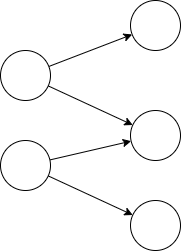
\includegraphics[scale=0.5]{img/sparsity.png}
	\caption{Išretinta sąveika}
	\label{img:sparsity}
\end{figure}

Dėl išretintos sąveikos konvoliuciniai neuroniniai tinklai atsižvelgia tik į reikšmingus požymius. Todėl konvoliucinių neuroninių tinklų mokymas trunka trumpiau ir triukšmas turi mažesnę įtaką rezultatui.

Kitas principas dėl kurio konvoliuciniai neuroniniai tinklai yra spartesni nei daugiasluoksniai perceptronai yra parametrų pasidalinimas. Parametrų pasidalinimas - tai principas, kuriuo remiantis bent vienas parametras yra panaudojamas daugiau nei vienai funkcijai. Konvoliucinių neuroninių tinklų atveju kiekvienas branduolio narys yra naudojamas kiekvienam įvesties nariui.

\subsubsection{Konvoliucinio neuroninio tinklo sluoksnių tipai}

Konvoliucinio neuroninio tinklo sluoksniai yra skirstomi į tipus. Pagrindinis konvoliucinio neuroninio tinklo sluoksnio tipas yra konvoliucijos sluoksnis. 

% cont from 30 slide
\subsubsection{Daugiavaizdis konvoliucinis neuroninis tinklas}

Daugiavaizdis konvoliucinis neuroninis tinklas yra aprašytas darbe \cite{cnnExp1}. Daugiavaizdis konvoliucinis neuroninis tinklas - tai konvoliucinis neuroninis tinklas, turintis vieną vaizdų sujungimo sluoksnį (angl. view pooling layer). Vaizdų sujungimo sluoksnis - tai sluoksnis, kuriame kiekvieno duomenų rinkinio požymių žemėlapių rinkiniai, vadinami vaizdais, yra apjungiami. Vaizdų apjungimas yra atliekamas padalinant visus vaizdus į grupes su nurodytu tuo pačiu dydžiu, ir išsirenkant iš kiekvienos grupės po tiksliausią požymių žemėlapių rinkinį.

Daugiavaizdžio konvoliucinio neuroninio tinklo apmokymas vyksta dvejais etapais. Pirmasis etapas yra pasirinkto konvoliucinio neuroninio tinklo apmokymas. Tada antrasis etapas yra vaizdų apjungimo sluoksnio įterpimas ir apmokymo pratęsimas. Šis sluoksnis padalina apmokytą konvoliucinį neuroninį tinklą į du tinklus $C_1$ ir $C_2$. Tęsiant apmokymą, kiekviena 2D nuotrauka atskirai pereis $C_1$ tinklą. Tada vaizdų apjungimo sluoksnyje šios nuotraukos bus apjungiamos. Pabaigoje vaizdų apjungimo sluoksnio rezultatas pereis tinklą $C_2$. Daugiavaizdis konvoliucinis neuroninis tinklas yra atvaizduotas paveikslėlyje \ref{img:mvcnn}.

\begin{figure}[H]
	\centering
	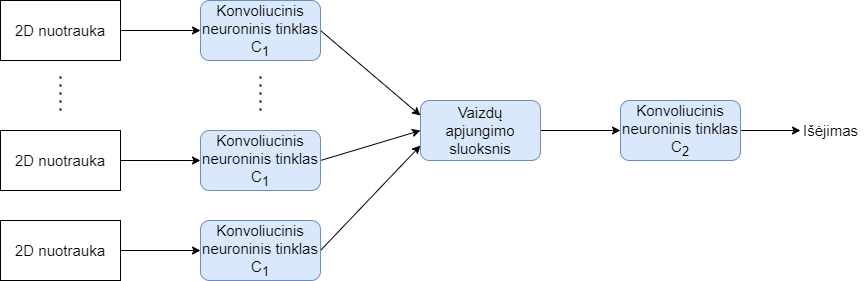
\includegraphics[scale=0.5]{img/mvcnn.png}
	\caption{Daugiavaizdis konvoliucinis neuroninis tinklas}
	\label{img:mvcnn}
\end{figure}

Darbo \cite{cnnExp1} autoriai teigia, kad teoriškai vaizdų apjungimo sluoksnį galima įterpti į bet kurią apmokyto konvoliucinio tinklo vietą. Tačiau šiame darbe atlikti tyrimai parodė, kad didžiausias tikslumas yra pasiekiamas įterpus šį sluoksni šalia paskutinio konvoliucijos sluoksnio.

% naudoti sv cnn - vggnet11
Darbe \cite{cnnExp1} aprašytas daugiavaizdis konvoliucinis neuroninis tinklas pirmame apmokymo etape naudoja VGG-M architektūra, kuri yra aprašyta darbe \cite{vggM}. Tačiau darbe \cite{cnnExp2} yra pasirinkta VGG-11 architektūra ir darbe \cite{cnnExp2} atliktame tyrime  daugiavaizdis konvoliucinis neuroninis tinklas pasiekė šiek tiek geresnius rezultatus. VGG-11 architektūra yra aprašyta darbe \cite{vgg11}. Šios architektūros konfigūracija yra atvaizduota lentelėje \ref{tbl:vgg11}. VGG-11 architektūroje po kiekvieno konvoliucijos ir pilnai sujungto sluoksnio, išskyrus paskutinio, tolimesnis sluoksnis yra apjungtas netiesiškumo ir ištaisymo sluoksnis su ištaisymo tiesine aktyvacijos funkcija. Tad, tam kad padaryti architektūros atvaizdavimą paprastesnį, šie sluoksniai nėra atvaizduoti lentelėje \ref{tbl:vgg11}. Po paskutinio pilnai sujungto sluoksnio tolimesnis sluoksnis yra netiesiškumo sluoksnis su softmax aktyvacijos funkcija. Taip pat šioje architektūroje visų konvoliucinių sluoksnių branduolių matmenys yra 3x3 ir lango žingsnis yra 1. Tuo metu visų sujungimo sluoksnių langų matmenys yra 2x2, lango žingsniai yra 2 ir visi sujungimo sluoksniai naudoja maksimalaus sujungimo metodą. Tad lentelėje \ref{tbl:vgg11} šie parametrai nėra atvaizduojami.

\begin{table}[h]
	\begin{tabular}{|l|c|l|}
		\hline
		Sluoksnio žymėjimas & Sluoksnio tipas            & \multicolumn{1}{c|}{Parametrai}       \\ \hline
		& Įėjimo sluoksnis           & Įėjimo matmenys = 224x224 RGB matrica \\ \hline
		$c_1$               & Konvoliucijos sluoksnis    & Branduolių skaičius = 64              \\ \hline
		$p_1$               & Sujungimo sluoksnis        &                                       \\ \hline
		$c_1$               & Konvoliucijos sluoksnis    & Branduolių skaičius = 128             \\ \hline
		$p_1$               & Sujungimo sluoksnis        &                                       \\ \hline
		$c_1$               & Konvoliucijos sluoksnis    & Branduolių skaičius = 256             \\ \hline
		$c_1$               & Konvoliucijos sluoksnis    & Branduolių skaičius = 256             \\ \hline
		$p_1$               & Sujungimo sluoksnis        &                                       \\ \hline
		$c_1$               & Konvoliucijos sluoksnis    & Branduolių skaičius = 512             \\ \hline
		$c_1$               & Konvoliucijos sluoksnis    & Branduolių skaičius = 512             \\ \hline
		$p_1$               & Sujungimo sluoksnis        &                                       \\ \hline
		$c_1$               & Konvoliucijos sluoksnis    & Branduolių skaičius = 512             \\ \hline
		$c_1$               & Konvoliucijos sluoksnis    & Branduolių skaičius = 512             \\ \hline
		$p_1$               & Sujungimo sluoksnis        &                                       \\ \hline
		$fc_1$              & Pilnai sujungtas sluoksnis & Neuronų skaičius = 4096               \\ \hline
		$fc_1$              & Pilnai sujungtas sluoksnis & Neuronų skaičius = 4096               \\ \hline
		$fc_1$              & Pilnai sujungtas sluoksnis & Neuronų skaičius = 1000               \\ \hline
		$fc_1$              & Pilnai sujungtas sluoksnis & Aktyvacijos funkcija - softmax        \\ \hline
	\end{tabular}
	\caption{VGG-11 architektūra}
	\label{tbl:vgg11}
\end{table}

Pirmame ir antrame apmokymo etape yra optimizuojama kryžminės entropijos nuostolių funkcija naudojantis Adam optimizavimo algoritmu. Antro etapo pradžioje vaizdų apjungimo sluoksnis yra įterpiamas tarp sluoksnių $p_5$ ir $fc_1$. Šio sluoksnio vaizdų grupių dydžiai yra lygūs 12.

% more info on research result or maybe write about it in research section?

\subsection{Kapsulinių dirbtinių neuroninių tinklų apžvalga}
Kapsuliniai neuroniniai tinklai yra aprašyti darbe \cite{capsNet}. Kapsuliniai neuroniniai tinklai yra giliųjų neuroninių tinklų tipas, kurio sluoksnio perceptronai yra grupuojami į kapsules. Kiekviena kapsulė apskaičiuoja tikimybę, kad paveikslėlyje pavaizduotas objektas priklauso kažkuriai klasei, ir išgauna informaciją apie tokius objekto bruožus kaip pozicija, orientacija, mastelis, deformacija, spalva ir kitus panašius objekto bruožus. Pirminių kapsulių sluoksnyje nagrinėjami objektai yra paprastos geometrinės figūros. Tolimesniuose sluoksniuose objektai darosi sudėtingesni, jie ima atitikti realaus pasaulio objektus. Kapsulės tarp sluoksnių yra sujungiamos į hierarchiją. Taip kapsulinis neuroninis tinklas sukuria hierarchinę vaizdo reprezentaciją.

Pirmieji du sluoksniai kapsuliniame neuroniniame tinkle yra konvoliucijos sluoksnis ir apjungtas netiesiškumo ir ištaisymo sluoksnis su ištaisymo tiesine aktyvacijos funkcija. Šių sluoksnių tikslas yra išgauti pagrindinius požymius, kurie tolimesniame sluoksnyje yra naudojami objektų konstrukcijai.

Tolimesnio sluoksnio tipas yra pirminių kapsulių sluoksnis (angl. primary capsules). Šiame sluoksnyje aktyvacijos žemėlapiai yra konvertuojami į vektorius. Toliau kiekvienas vektorius atskirai yra pateikiamas squash funkcijai kaip argumentai. Squash funkcija yra formulė (\ref{eqn:squash}), kur $||s||$ yra visų matricos $s$ narių suma.

\begin{equation}
\label{eqn:squash}
	squash(s) = \dfrac{||s||^2}{1 + ||s||^2}\dfrac{s}{||s||}
\end{equation}

Tolimesnių sluoksnių tipai yra kapsuliniai sluoksniai. Šiuose sluoksniuose yra vykdomas dinaminis maršrutizavimas tarp kapsulių (angl. dynamic routing between capsules). Dinaminis maršrutizavimas tarp kapsulių - tai iteratyvus procesas, kurio paskirtis yra apjungti kapsules tarp dviejų sluoksnių. Prieš pradedant iteratyvią proceso dalį, kiekvienai sluoksnio $l$ kapsulei $i$ ir sluoksnio $(l + 1)$ kapsulei $j$ yra inicializuojami kintamieji $b_{ij}$ su reikšme 0. Taip pat kiekvienai kapsulių $i$ ir $j$ porai yra apskaičiuojami vektoriai $\hat{u}_{j|i}$ pagal formulę (\ref{eqn:pred_vectors}), kur $W_{ij}$ yra svorio matrica tarp kapsulių $i$ ir $j$ bei $u_{i}$ - tai kapsulės $i$ išvestis.

\begin{equation}
\label{eqn:pred_vectors}
	\hat{u}_{j|i} = W_{ij} u_{ij}
\end{equation}

Tada pirmasis iteratyvaus proceso žingsnis yra apskaičiuoti apjungimo koeficientus $c_{ij}$ kiekvienai kapsulių $i$ ir $j$ porai pagal softmax funkciją atvaizduota formulėje (\ref{eqn:coupling_coef}), kur $n$ yra sluoksnio $(l + 1)$ kapsulių skaičius.

\begin{equation}
\label{eqn:coupling_coef}
	c_{ij} = \dfrac{\exp^{b_{ij}}}{\sum_{k = 1}^{n} \exp^{b_{ik}}}
\end{equation}

Tolimesnis žingsnis yra apskaičiuoti svertines sumas $s_j$ kiekvienai kapsulei $j$ naudojantis formulę (\ref{eqn:weighted_sum}), kur $m$ yra kapsulių skaičius sluoksnyje $l$.

\begin{equation}
\label{eqn:weighted_sum}
	s_{j} = \sum_{i = 1}^{m} c_{ij} \hat{u}_{j|i}
\end{equation}

Toliau yra apskaičiuojami vektoriai $v_j$ kiekvienai kapsulei $j$ naudojantis softmax funkcija su argumentu $s_j$. Kitaip tariant yra apskaičiuojama formulė $v_j = softmax(s_j)$. Paskutinis iteratyvios dalies žingsnis yra pakeisti kintamųjų $b_{ij}$ reikšmes naudojantis formulę $b_{ij} = b_{ij} + \hat{u}_{j|i} v_j$.

Iteratyvi dinaminio maršrutizavimo tarp kapsulių proceso dalis yra kartojama nurodyta skaičių iteracijų ir šio proceso rezultatas yra vektorius $v_j$. Šiame vektoriuje yra tikimybės, kad objektas, nagrinėjamas kapsulės $i$, yra dalis objekto, nagrinėjamo kapsulės $j$. Paskutinio kapsulinio sluoksnio kapsulės nagrinėja klases.

Po visų kapsulinių sluoksnių kapsuliniame neuroniniame tinkle yra naudojamas rekonstrukcijos tinklas. Rekonstrukcijos tinklas yra sudarytas iš 3 sluoksnių. Du pirmieji sluoksniai yra apjungti netiesiškumo ir ištaisymo sluoksniai su ištaisymo tiesine aktyvacijos funkcija. Paskutinis sluoksnis yra netiesiškumo sluoksnis  su sigmoidine aktyvacijos funkcija. Šio tinklo uždavinys yra atkurti įėjimo 2D nuotrauką. Tad kapsulinio neuroninio tinklo išėjimo sluoksnio rezultatas yra ne tik priskirta klasė, bet ir atkurta įėjimo reikšmė.

Kapsulinis neuroninis tinklas yra apmokomas optimizuojant 2 funkcijas. Pirmoji funkcija yra margin nuostolių funkcija, pavaizduota formulėje (\ref{eqn:margin_loss}), kur $L_k$ yra funkcijos rezultatas kapsulei $k$, $||v_k||$ - visų kapsulės $k$ išėjimo $v_k$ narių suma, $T_k$ konstanta lygi 1 jei įėjimui yra priskirta klasė, kuri yra nagrinėjama kapsulėje $k$, kitu atveju - 0, $m^+ = 0.9$, $m^- = 0.1$ ir $\lambda$ yra nurodyta konstanta, skirta mažinti neteisingų klasių įtaką, šiame magistro baigiamajame darbe $\lambda = 0.5$.

\begin{equation}
\label{eqn:margin_loss}
	L_{k} = T_k max(0, m^+ - ||v_k||)^2 + \lambda (1 - T_k) max(0, ||v_k|| - m^-)^2
\end{equation}

Antroji nuostolių funkcija yra rekonstrukcijos nuostolių funkcija $RL$. Ši funcija yra vidutinė kvadratinė paklaida (angl. mean square error) tarp atkurtos įėjimo matricos ir originalios įėjimo matricos. Apmokyme šios 2 funkcijos yra apjungtos į funkciją pavaizduota formulėje (\ref{eqn:total_margin_loss}), kur $n$ yra klasių skaičius ir $\alpha$ - tai rekonstrukcijos nuostolių funkcijos įtakos mažinimo konstanta, šiame magistro baigiamajame darbe $\alpha = 0.0005$.

\begin{equation}
\label{eqn:total_margin_loss}
	TL = \sum_{k = 1}^{n} L_{k} + \alpha RL
\end{equation}


\section{Kapsulinių neuroninių tinklų modifikacijos ir parametrai}

\section{Eksperimentiniai tyrimai}

\subsection{Tyrimams naudoti duomenys}

\subsection{Kapsulinių neuroninių tinklų modifikacijų ir parametrų eksperimentiniai tyrimai}

\subsection{Kapsulinių ir daugiavaizdžių konvoliucinių neuroninių tinklų eksperimentiniai tyrimai}

Šiame magistro baigiamame darbe yra palyginami 4 neuroninių tinklų architektūros: daugiavaizdis neuroninis tinklas, aprašytas poskyryje Daugiavaizdis konvoliucinis neuroninis tinklas, kapsulinis neuroninis tinklas, aprašytas poskyryje Tiriamo kapsulinio neuroninio tinklo architektūra, ir 2 daugiavaizdžiai kapsuliniai neuroniniai tinklai, aprašyti poskyriuose Tiriamo daugiavaizdžio kapsulinio neuroninio tinklo architektūra su vaizdų sujungimo sluoksniu ir Tiriamo daugiavaizdžio kapsulinio neuroninio tinklo architektūra su vaizdų kapsuliniu sluoksniu. Kiekvienas tiriamas dirbtinis neuroninis tinklas yra apmokomas naudojantis visais duomenimis, aprašytais poskyryje Tyrimams naudoti duomenys. Šie duomenys apmokymo metu yra padalinami į duomenų rinkinius, kurių dydžiai yra 96. Daugiavaizdžio konvoliucinio ir kapsulinio neuroninių tinklų apmokymų antram etapui duomenų rinkiniai sudaryti iš nuotraukų grupių, kuriose yra visos konkretaus 3D objekto modelio nuotraukos. Kiekvienas dirbtinis neuroninis tinklas yra apmokomas per 10 epochų. Daugiavaizdžio konvoliucinio ir kapsulinio neuroninių tinklų abu apmokymo etapai yra apmokomi po 5 epochas. Visų šiame magistro baigiamame darbe tiriamų dirbtinių neuroninių tinklų apmokymai trunka po 6-7 valandas naudojantis Kaggle sistema.

Šiame magistro baigiamame darbe bandoma optimizuoti kapsulinių neuroninių tinklų modifikacijų konfigūracijas. Pirmiausia bandoma optimizuoti šiuos tinklus naudojantis Bajeso hiperparametrų optimizavimo algoritmu, kuris yra aprašytas darbe \cite{bayes}. Toliau bandomos kitos konfigūracijos nei konfigūracijos aprašytos darbe \cite{capsNet}. Tačiau, dėl Kaggle sistemos apribojimų, nei vienas metodas neaptiko geresnių kapsulinių neuroninių tinklų modifikacijų konfigūracijų. Taip pat bandoma 
keisti mokymosi greitį. Tačiau skirtumai tarp rezultatų yra nereikšmingi.

Po kiekvienos epochos yra renkamos tikslumo metrikos: tikslumas klasifikuojant apmokymo duomenis, ši informacija pavaizduota lentelėje \ref{tbl:train} ir grafe \ref{img:train_plot}, ir tikslumas klasifikuojant testavimo duomenis, ši informacija atvaizduota lentelėje \ref{tbl:valid} ir grafe \ref{img:val_plot}. Tikslumas yra teisingai suklasifikuotų įrašų dalis klasifikuotų duomenų aibėje. Lentelių \ref{tbl:train}, \ref{tbl:valid} stulpelio pavaidinimas ir grafų \ref{img:train_plot}, \ref{img:val_plot} kreivių pavadinimas mvcnn yra daugiavaizdžio neuroninio tinklo tikslumas, capsnet - kapsulinio neuroninio tinklo tikslumas, mv\_capsnet - daugiavaizdžio kapsulinio neuroninio tinklo su vaizdų sujungimo sluoksniu tikslumas, mv\_cap\_capsnet1 - daugiavaizdžio kapsulinio neuroninio tinklo su vaizdų kapsuliniu sluoksniu ir vienu mokymosi etapu tikslumas, mv\_cap\_capsnet2 - daugiavaizdžio kapsulinio neuroninio tinklo su vaizdų kapsuliniu sluoksniu ir dviem mokymosi etapais tikslumas. Brūkšninė vertikali linija grafuose \ref{img:train_plot} ir \ref{img:val_plot} nurodo antrojo apmokymo etapo pirmąją epochą.

\begin{table}[]
\begin{tabular}{l|l|l|l|l|l}
	epocha &     mvcnn &   capsnet & mv\_capsnet & mv\_cap\_capsnet1 & mv\_cap\_capsnet2 \\ \hline
	0 &  0.687898 &  0.119029 &   0.517437 &        0.281199 &        0.217937 \\
	1 &  0.859519 &  0.528616 &   0.793225 &        0.806504 &        0.624331 \\
	2 &  0.903853 &  0.660332 &   0.840396 &        0.879980 &        0.731115 \\
	3 &  0.928760 &  0.719580 &   0.871316 &        0.911382 &        0.785434 \\
	4 &  0.944097 &  0.757512 &   0.895495 &        0.933435 &        0.820672 \\
	5 &  0.937398 &  0.783308 &   0.878354 &        0.947866 &        0.717276 \\
	6 &  0.949593 &  0.804666 &   0.928862 &        0.957927 &        0.910976 \\
	7 &  0.958740 &  0.821037 &   0.952439 &        0.965447 &        0.944411 \\
	8 &  0.961077 &  0.834765 &   0.965854 &        0.970427 &        0.961992 \\
	9 &  0.971951 &  0.847070 &   0.972459 &        0.974594 &        0.969614 \\
	
\end{tabular}
\caption{
	Apmokymo duomenų klasifikavimo tikslumas, kur mvcnn yra daugiavaizdžio neuroninio tinklo tikslumas, capsnet - kapsulinio neuroninio tinklo tikslumas, mv\_capsnet - daugiavaizdžio kapsulinio neuroninio tinklo su vaizdų sujungimo sluoksniu tikslumas, mv\_cap\_capsnet1 - daugiavaizdžio kapsulinio neuroninio tinklo su vaizdų kapsuliniu sluoksniu ir vienu mokymosi etapu tikslumas, mv\_cap\_capsnet2 - daugiavaizdžio kapsulinio neuroninio tinklo su vaizdų kapsuliniu sluoksniu ir dviem mokymosi etapais tikslumas.
}
\label{tbl:train}
\end{table}

\begin{table}[]
\begin{tabular}{l|l|l|l|l|l}
	epocha &     mvcnn &   capsnet & mv\_capsnet & mv\_cap\_capsnet1 & mv\_cap\_capsnet2 \\ \hline
	0 &  0.791531 &  0.302292 &   0.718333 &        0.691558 &        0.479573 \\
	1 &  0.835160 &  0.561875 &   0.768125 &        0.788961 &        0.629025 \\
	2 &  0.849466 &  0.630833 &   0.777917 &        0.821834 &        0.687466 \\
	3 &  0.857515 &  0.663125 &   0.783958 &        0.828328 &        0.714421 \\
	4 &  0.859916 &  0.683125 &   0.800417 &        0.850244 &        0.721354 \\
	5 &  0.888393 &  0.674167 &   0.800000 &        0.861201 &        0.831981 \\
	6 &  0.880276 &  0.698333 &   0.822500 &        0.864448 &        0.848214 \\
	7 &  0.881088 &  0.701250 &   0.827500 &        0.862013 &        0.838068 \\
	8 &  0.896104 &  0.722917 &   0.807500 &        0.861201 &        0.840503 \\
	9 &  0.900974 &  0.710417 &   0.852500 &        0.855925 &        0.827516 \\
	
\end{tabular}
\caption{
	Testavimo duomenų klasifikavimo tikslumas, kur mvcnn yra daugiavaizdžio neuroninio tinklo tikslumas, capsnet - kapsulinio neuroninio tinklo tikslumas, mv\_capsnet - daugiavaizdžio kapsulinio neuroninio tinklo su vaizdų sujungimo sluoksniu tikslumas, mv\_cap\_capsnet1 - daugiavaizdžio kapsulinio neuroninio tinklo su vaizdų kapsuliniu sluoksniu ir vienu mokymosi etapu tikslumas, mv\_cap\_capsnet2 - daugiavaizdžio kapsulinio neuroninio tinklo su vaizdų kapsuliniu sluoksniu ir dviem mokymosi etapais tikslumas.	
}
\label{tbl:valid}
\end{table}

\begin{figure}[H]
	\centering
	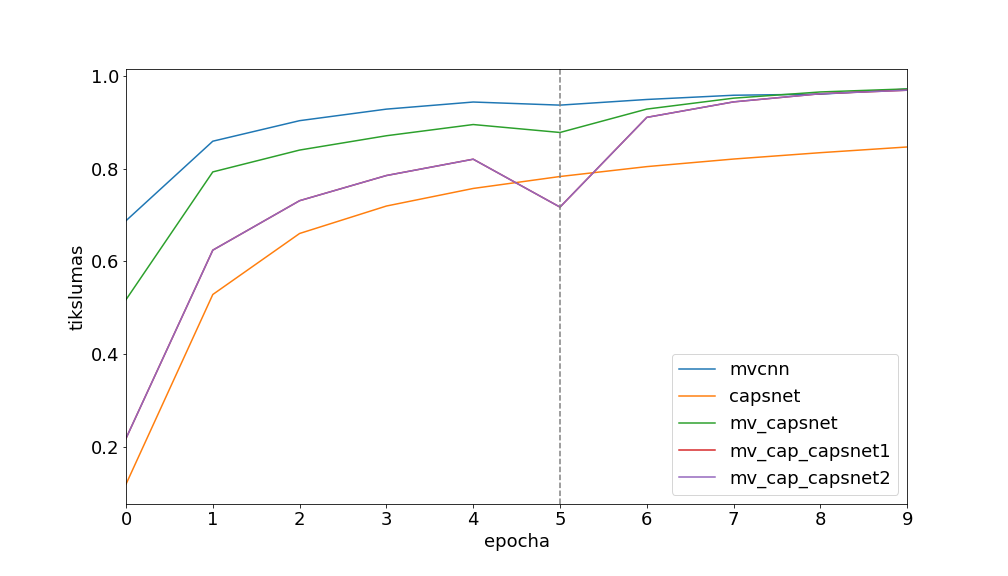
\includegraphics[scale=0.5]{img/trained.png}
	\caption{
		Apmokymo duomenų klasifikavimo tikslumas, kur mvcnn yra daugiavaizdžio neuroninio tinklo tikslumas, capsnet - kapsulinio neuroninio tinklo tikslumas, mv\_capsnet - daugiavaizdžio kapsulinio neuroninio tinklo su vaizdų sujungimo sluoksniu tikslumas, mv\_cap\_capsnet1 - daugiavaizdžio kapsulinio neuroninio tinklo su vaizdų kapsuliniu sluoksniu ir vienu mokymosi etapu tikslumas, mv\_cap\_capsnet2 - daugiavaizdžio kapsulinio neuroninio tinklo su vaizdų kapsuliniu sluoksniu ir dviem mokymosi etapais tikslumas. Brūkšninė vertikali linija nurodo antrojo apmokymo etapo pirmąją epochą.
	}
	\label{img:train_plot}
\end{figure}

\begin{figure}[H]
	\centering
	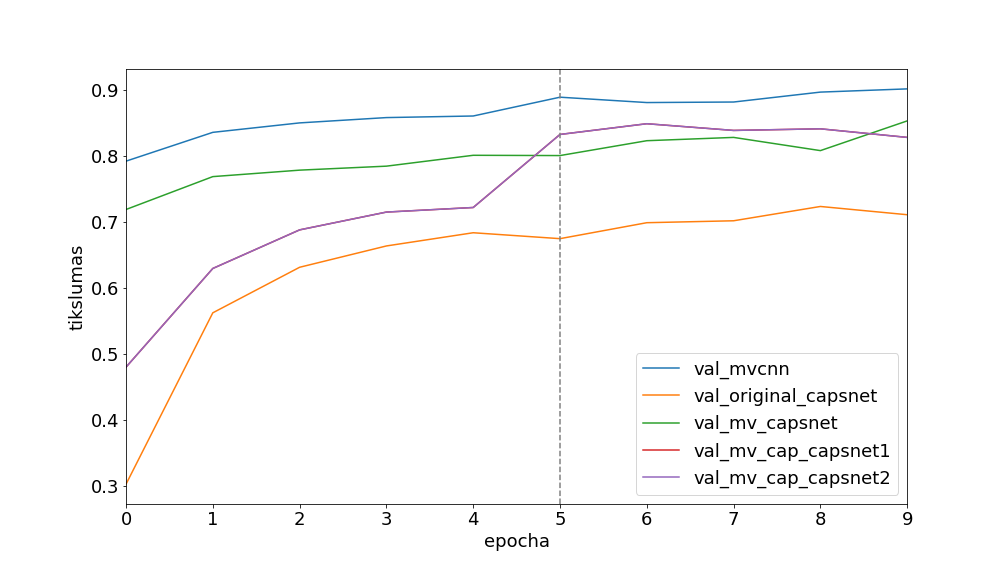
\includegraphics[scale=0.5]{img/validated.png}
	\caption{
		Testavimo duomenų klasifikavimo tikslumas, kur mvcnn yra daugiavaizdžio neuroninio tinklo tikslumas, capsnet - kapsulinio neuroninio tinklo tikslumas, mv\_capsnet - daugiavaizdžio kapsulinio neuroninio tinklo su vaizdų sujungimo sluoksniu tikslumas, mv\_cap\_capsnet1 - daugiavaizdžio kapsulinio neuroninio tinklo su vaizdų kapsuliniu sluoksniu ir vienu mokymosi etapu tikslumas, mv\_cap\_capsnet2 - daugiavaizdžio kapsulinio neuroninio tinklo su vaizdų kapsuliniu sluoksniu ir dviem mokymosi etapais tikslumas. Brūkšninė vertikali linija nurodo antrojo apmokymo etapo pirmąją epochą.
	}
	\label{img:val_plot}
\end{figure}


\sectionnonum{Rezultatai ir išvados}

Šiame magistro baigiamame darbe atlikta:

\begin{enumerate}
	\item Aprašytos ir realizuotos kapsulinių neuroninių tinklų dvi modifikacijos - daugiavaizdžiai kapsuliniai neuroniniai tinklai, iš kurių su vienas yra su vaizdų sujungimo sluoksniu ir kitas su vaizdų kapsuliniu sluoksniu.
	\item Atlikti tyrimai skirti nustatyti geriausią kapsulinių neuroninių tinklų modifikacijų konfigūracijas ir palyginti jas su nemodifikuotu kapsuliniu neuroniniu tinklu.
	\item Atlikti tyrimai, skirti palyginti kapsulinių neuroninių tinklų modifikacijas su dabartiniu geriausiu daugiavaizdžiu konvoliuciniu neuroniniu tinklu.
\end{enumerate}

Atlikus tyrimus šiame magistro baigiamame darbe gautos tokios išvados:

\begin{enumerate}
	\item Atlikti eksperimentiniai tyrimai su pilna duomenų imtimi indikuoja, kad daugiavaizdžiai kapsuliniai neuroniniai tinklai pasiekia geresnius rezultatus per panašų apmokymo laiką nei kapsuliniai neuroniniai tinklai.
	\item Taip pat šie tyrimai indikuoja, kad daugiavaizdžiai kapsuliniai neuroniniai tinklai su vaizdų kapsuliniu sluoksniu yra pranašesnis tikslumo atžvilgiu už daugiavaizdžį kapsulinį neuroninį tinklą su vaizdų sujungimo sluoksniu.
	\item Tyrimai su pilna duomenų imtimi indikuoja, kad daugiavaizdžio kapsulinio neuroninio tinklo su vaizdų kapsuliniu sluoksniu, apmokant jį su vienu etapu, tikslumas pradeda konverguoti greičiau nei apmokant jį dvejais etapais. Tad šios daugiavaizdžio kapsulinio neuroninio tinklo modifikacijos apmokymas su vienu etapu yra pranašesnis laiko atžvilgiu už apmokymą su dvejais etapais.
	\item Paskutinė išvada padaryta iš tyrimų su pilna duomenų imtimi yra, kad šie tyrimai indikuoja dabartinio geriausio daugiavaizdžio konvoliucinio neuroninio tinklo pranašumą prieš visas šiame magistro darbe tirtas kapsulinio neuroninio tinklo modifikacijas atsižvelgiant į tikslumo kriterijų.
	\item Tuo metu atlikti eksperimentai su mažesnėmis duomenų imtimis indikuoja, kad kuo mažesnė duomenų imtis, tuo skirtumas tarp daugiavaizdžio kapsulinio neuroninio tinklo su vaizdų kapsuliniu sluoksniu, kuris yra apmokomas vienu etapu, ir dabartinio geriausio daugiavaizdžio konvoliucinio neuroninio tinklo yra nereikšmingesnis.
\end{enumerate}

Daugiavaizdžiui konvoliuciniui neuroniniui tinklui yra sudėtinga pritaikyti vaizdų kapsulinį sluoksnį nepaverčiant jo daugiavaizdžiu kapsuliniu neuroniniu tinklu. Tačiau pirmieji kapsulinių neuroninių tinklų sluoksniai sudaro konvoliucinį neuroninį tinklą. Todėl egzistuoja galimybė apjungti VGG-11 architektūrą, kuri naudojama dabartinio geriausio daugiavaizdžio konvoliucinio neuroninio tinklo pirmojo etapo apmokyme, su daugiavaizdžiu kapsuliniu neuroniniu tinklu su vaizdų kapsuliniu sluoksniu. Tad ateityje reikia tyrimais palyginti šį apjungtą dirbtinį neuroninį tinklą su dabartiniu geriausiu daugiavaizdžiu konvoliuciniu neuroniniu tinklu.

Rezultatų ir išvadų dalyje išdėstomi pagrindiniai darbo rezultatai (kažkas
išanalizuota, kažkas sukurta, kažkas įdiegta), pateikiamos išvados (daromi
nagrinėtų problemų sprendimo metodų palyginimai, siūlomos rekomendacijos,
akcentuojamos naujovės).

\printbibliography[heading=bibintoc]  % Literatūros šaltiniai aprašomi
% bibliografija.bib faile. Šaltinių sąraše nurodoma panaudota literatūra,
% kitokie šaltiniai. Abėcėlės tvarka išdėstoma tik darbe panaudotų (cituotų,
% perfrazuotų ar bent paminėtų) mokslo leidinių, kitokių publikacijų
% bibliografiniai aprašai (šiuo punktu pasirūpina LaTeX). Aprašai pateikiami
% netransliteruoti.

% \sectionnonum{Sąvokų apibrėžimai}
\sectionnonum{Santrumpos}
Sąvokų apibrėžimai ir santrumpų sąrašas sudaromas tada, kai darbo tekste
vartojami specialūs terminai, reikalaujantys paaiškinimo, ir rečiau sutinkamos
santrumpos.

\appendix  % Priedai
% Prieduose gali būti pateikiama pagalbinė, ypač darbo autoriaus savarankiškai
% parengta, medžiaga. Savarankiški priedai gali būti pateikiami kompiuterio
% diskelyje ar kompaktiniame diske. Priedai taip pat vadinami ir numeruojami.
% Tekstas su priedais siejamas nuorodomis.

\section{Niauroninio tinklo struktūra}

\section{Eksperimentinio palyginimo rezultatai}
% tablesgenerator.com - converts calculators (e.g. excel) tables to LaTeX
\begin{table}[H]\footnotesize
  \centering
  \caption{Lentelės pavyzdys}
  {\begin{tabular}{|l|c|c|} \hline
    Algoritmas & $\bar{x}$ & $\sigma^{2}$ \\
    \hline
    Algoritmas A  & 1.6335    & 0.5584       \\
    Algoritmas B  & 1.7395    & 0.5647       \\
    \hline
  \end{tabular}}
  \label{tab:table example}
\end{table}

\end{document}
